\section{Episode 47: Emancipation, Preparation, Consternation and Anticipation!}

\medskip

\DndDropCapLine{B}\textit{urnies left arm begins twitching uncontrollably, where burnie lies in an orc-meat induced coma, it manages to grab a pen, and begins scrawling in a nearby open file.} \medskip

Hi There! I’m Mark, Mark o’Synne! I’m currently trapped in the arm of a non-magical curmudgeon, so this is kind of a difficult task of me. Seems I can only write things when he’s in a proto-canabalistic food comer. Cool! Maybe I’ll manifest soon, once I’ve gathered enough latent magical energy, but til then I’ll just make do, longing for some sort of wrist-worn time-piece! Anyway, I have a prediction, my existence at the moment puts me slightly outside the chrono-stream, and I’m pretty sure I should warn them all of the horrors of what’s going to happen!\medskip

Anyway, I betcha everyone will get woken up, and confusedly send Kolo to meet with lady Imicha - they’ll sort it before they all end up together. Kolo and the gang give their appraisal of the situation in, what we call in hell, a “shit sandwich” of good news! Seems that the Masudan army have been using guns, which is less than good, but Kolo is awesome and Riphard has a fancy cloak. Plus one less brother’s army to contend with - all round good news! Oh, yeah, the guns. And an army of about 500, in a heavily fortified city, with guns.\medskip

Exme demonstrates everything through the use of a rabbit flipbook, getting shot by a little Masudan man with a musket - excellent use of an animated medium, for I know it will be so! Oh god, I don’t even have a nose at the moment - but that orc-meat fart is horrendous! We’ll plan to use trebuchets…. No, Conrad, he can help us. Someone stands and accuses the goblins of being, well, goblins. Burnie throws a knife at his head, but misses burying it just beside his ear. The point is made - unfortunately in the beautiful theatre’s wall. The goblins put on a play. It’s a bit derivative. And no-one speaks the language. Kolo hams it up, not believable as the character.\medskip

Short version (mercifully) - Conrad builds robots, and the Geisha’s get their freedom - in order to all help. Riphard uses finger guns, which is weirdly persuasive enough to convince Imicho to send Lord Ko’nquo with us to pick up the murder bots. Exme comes up with all the ideas to outfit our ship with bombs and awesomeness. Geisha’s ability to pulverise chairs is revealed, as well as their well-known capacity for opening pickle jars. It’s a bit polarising display, but people are impressed, if concerned. As Riphard puts it “if you have a land of murder-robots, better to have them on your good side”. Burnie screams “Fer freedom”. If I could blush from embarrassment, I would.\medskip

We bump into Myron outside, and we’re worried that Riphard is trying to buy 100’000’s worth of Robots with 120’000’s worth of gold, shortchanging lady Imicha. Burnie Pigs ears for a cocktail, “The Swines Concerto”. It’s served in a pigs ear, gives it a nice waxy flavour. We end up back on the boat, making preparation to return to Conrad, along with our friend Lord Cumquat. Kolo breaks into Burnie’s room, and steals his files - but man-handles his bits in search of gold. Burnie Catches him, and dangles him out the door, before going to bed - but didn’t realise his files were gone. Kolo’s thinks he’s a little monster. Exme’s says she’s an angel, potential evil genius, but gold star appraisal overall. They build a smoke machine. And other stuff. New plan - load Daddy-Gary’s body into the smoke machine and get the whole city stoned!\medskip

We get to Conrads, and we talk to the Geisha’s, they’re happy about being emancipated! God he’s camp. I may have the relative form of a halfling, but I feel some short-person shame because of him. For Synne’s sake reel it in man! Lord whatsit and Conrad meet up, and start negotiating objects for the war effort. We have a big ol’ party, involving booze, and fireworks, and geisha, and fun, and booze. They reach an agreement! The Geisha’s get a stipend, and Riphard agrees, in his most noble way, to take Otarios - which is agreed!\medskip

Everyone mucks down to do some combat so conrad can work out how we all attack, to train the robots. Burnie dodges, Myron gets whipped and then shot (by Riphard), and Kolo is a dick. Gnomes don’t like Bum Play, but they do like healing shocker gauntlets! Myron and delilah and… Rip? Go to collect balloon cows. It’s more like bobbing for cows, or Myron impossible. Myron catches a cow, and Riphard lets of a celebratory gunshot. The balloon cows bloat, and they successfully(?) catch 3 of the little bastards.\medskip

Preparations continue, Myron foots in mouth (and so does Burnie) about the fact we don’t care about Masuda and just want the artefact, to the Geishas, they’re less than impressed. We’re here to get the hammer of the gods - I remember this thing! Can harm those enhanced by the power of Inthum, so pretty good against the Inquisition. The Geisha tell us the golden hall - basically a history museum of awesome loot - contains the hammer. Tall, likely gold, lit up with torches. We make our way on the airship, trying to sort out the best method of assault. General idea is using the airship to blow a hole to the city, get in, then using the ship to escape from the city. With a hold full of robots, and several magic bombs made by the terrible twins, and half an idea involving balloon cows and strafing strikes of bombing runs. Ah, CURSE my precognition… It’s premature!\medskip

I guess the exciting thing was going to happen next time! The damned bastard is waking up, so I better make myself scarce, saying that, sounds like Kolo will steal this file before Burnie ever sees it, so this flap of a butterfly’s wing won’t affect the ripples of time! Toodles!\medskip

Credit song: https://youtu.be/2c1iSpk3u1A (I dunno, it's catchy and just how I imagine us bimbling around in the flying machine)\medskip




\vspace*{5mm}

\begin{center}
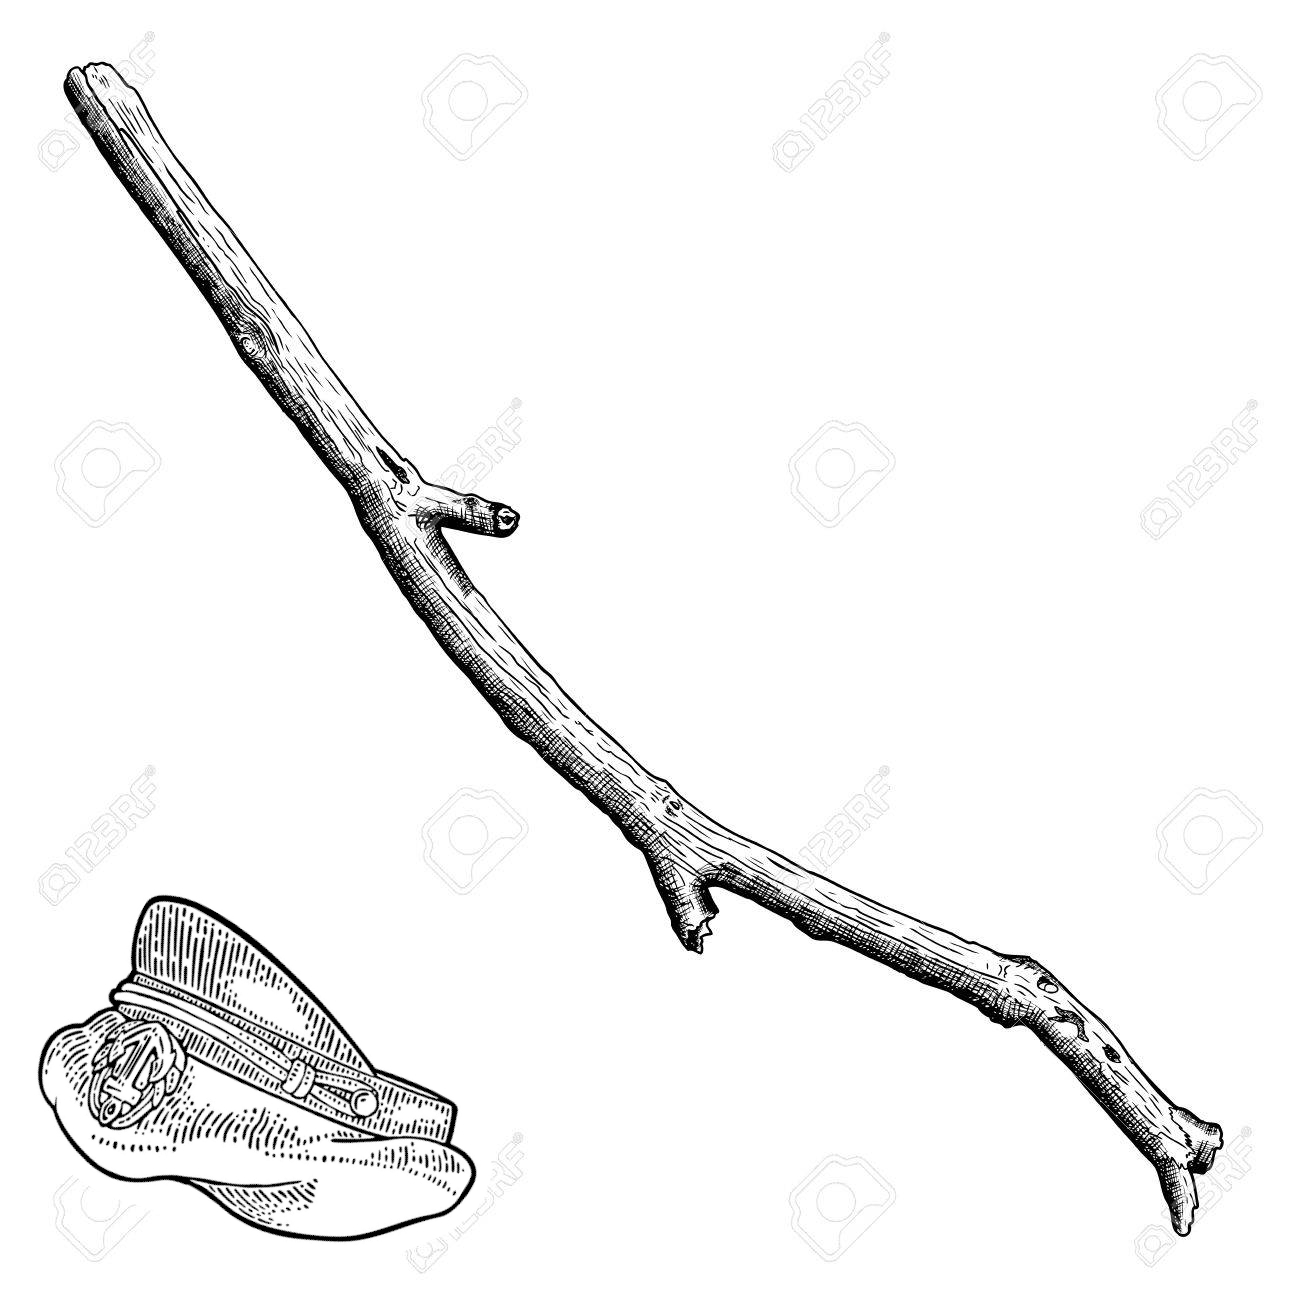
\includegraphics[width=\textwidth]{./content/img/xxx.jpg}
\begin{figure}[h]
\end{figure}
\end{center}

\clearpage